\documentclass[a4paper]{extarticle}
\usepackage[utf8]{inputenc}
\usepackage[a4paper, margin=1in]{geometry}

\usepackage{amssymb}
\usepackage{amsmath}
\usepackage{enumitem}
\usepackage{tcolorbox}
\usepackage{fancyhdr}
\usepackage{graphicx}
\usepackage{float}

\setlength{\parindent}{0em}
\setlength{\parskip}{0.4em}

\definecolor{theoremblue}{RGB}{1, 73, 124}
\definecolor{corollaryblue}{RGB}{70, 143, 175}
\definecolor{exampleblue}{RGB}{137, 194, 217}

\newtcolorbox{tbox}{colback=theoremblue!20,colframe=theoremblue,
boxrule=0pt,arc=0pt,boxsep=2pt,left=2pt,right=2pt,leftrule=2pt}

\newtcolorbox{cbox}{colback=corollaryblue!20,colframe=corollaryblue,
boxrule=0pt,arc=0pt,boxsep=2pt,left=2pt,right=2pt,leftrule=2pt}

\newtcolorbox{ebox}{colback=exampleblue!20,colframe=exampleblue,
boxrule=0pt,arc=0pt,boxsep=2pt,left=2pt,right=2pt,leftrule=2pt}

\title{EnpRisk - Lecture Notes Week 10}
\author{Ruben Schenk, ruben.schenk@inf.ethz.ch}
\date{\today}

\pagestyle{fancy}
\fancyhf{}
\rhead{ruben.schenk@inf.ethz.ch}
\rfoot{Page \thepage}
\lhead{EnpRisk - Lecture Notes Week 10}

\begin{document}

\maketitle

\subsection{Conclusion}

It is important to stress that we view this cycle as \textbf{endogenous.} Boom and bust are two sides of the same coin. It is a fundamental property of capitalism to cycle through periods of optimism and pessimism. Periods of growth have the tendency to \textit{overshoot.} This is naturally corrected in a phase of consolidation or even decline.

This is in stark contrast to the \textbf{exogenous} view, where recessions are seen as a symptom of disease, caused by some external factor that needs to be eradicated or modified for the system to be cured.

According to Hyman Minsky, capitalism has evolved, since the late nineteenth century, through a \textit{super-financial business cycle} with four stages:

\paragraph{Commercial capitalism} In commercial capitalism, the financial system was centered around commercial banks. Banks financed \textit{working capital,} in the form of short-term loans, to cover operational expenditures and the purchase of materials necessary in the production process. Long-term investments were financed from retained profits, or from equity injected by the owners.

\paragraph{Financial capitalism} The second industrial revolution drastically changed the system: With the need to build big infrastructure came the strong demand for the long-term financing of \textit{capital expenditure (CAPEX).} Finance became globalized as stocks and bonds, issued to service long-term capital investments, were sold in international financial markets. The financial system became dominated by \textit{investment banks.} As Minsky said: "\textit{Stability is destabilizing.}" By the 1920s, investment banks were largely devoting their effort to financing speculation in financial assets. As such, "finance capitalism" ended in the crash of 1929, which ultimately lead to the Great Depression.

\paragraph{Managerial welfare capitalism} After the 1929 crash and during the Great Depression, the pendulum swung back. The financial sector was reformed with the New Deal legislation and the federal government took up a bigger role in managing the economy. Following the transition period, this corresponds to the Golden Age of stable economic growth, high employment and social contract between workers and owners. However, the absence of deep recession and severe financial crises encouraged innovations that increased instability. The New Deal reforms were cut back, and the financial system was again deregulated.

\paragraph{Money manager capitalism} The Golden Age created large pools of savings. From this, the \textbf{shadow banking system} was born (pension funds, asset manager, mutual funds, etc.). The reason of existence of this type of capitalism is to manage huge pools of capital in search of the highest returns. The financial system no longer serves the productive economy but serves only itself. The innovation and exploration process started focusing on the financial sector itself. This is what we call \textbf{financialization,} which lead to a massive growth in complex financial derivatives.

\textbf{Overview of the 150 years perspective on society, economy and technology:}

\begin{figure}[H]
    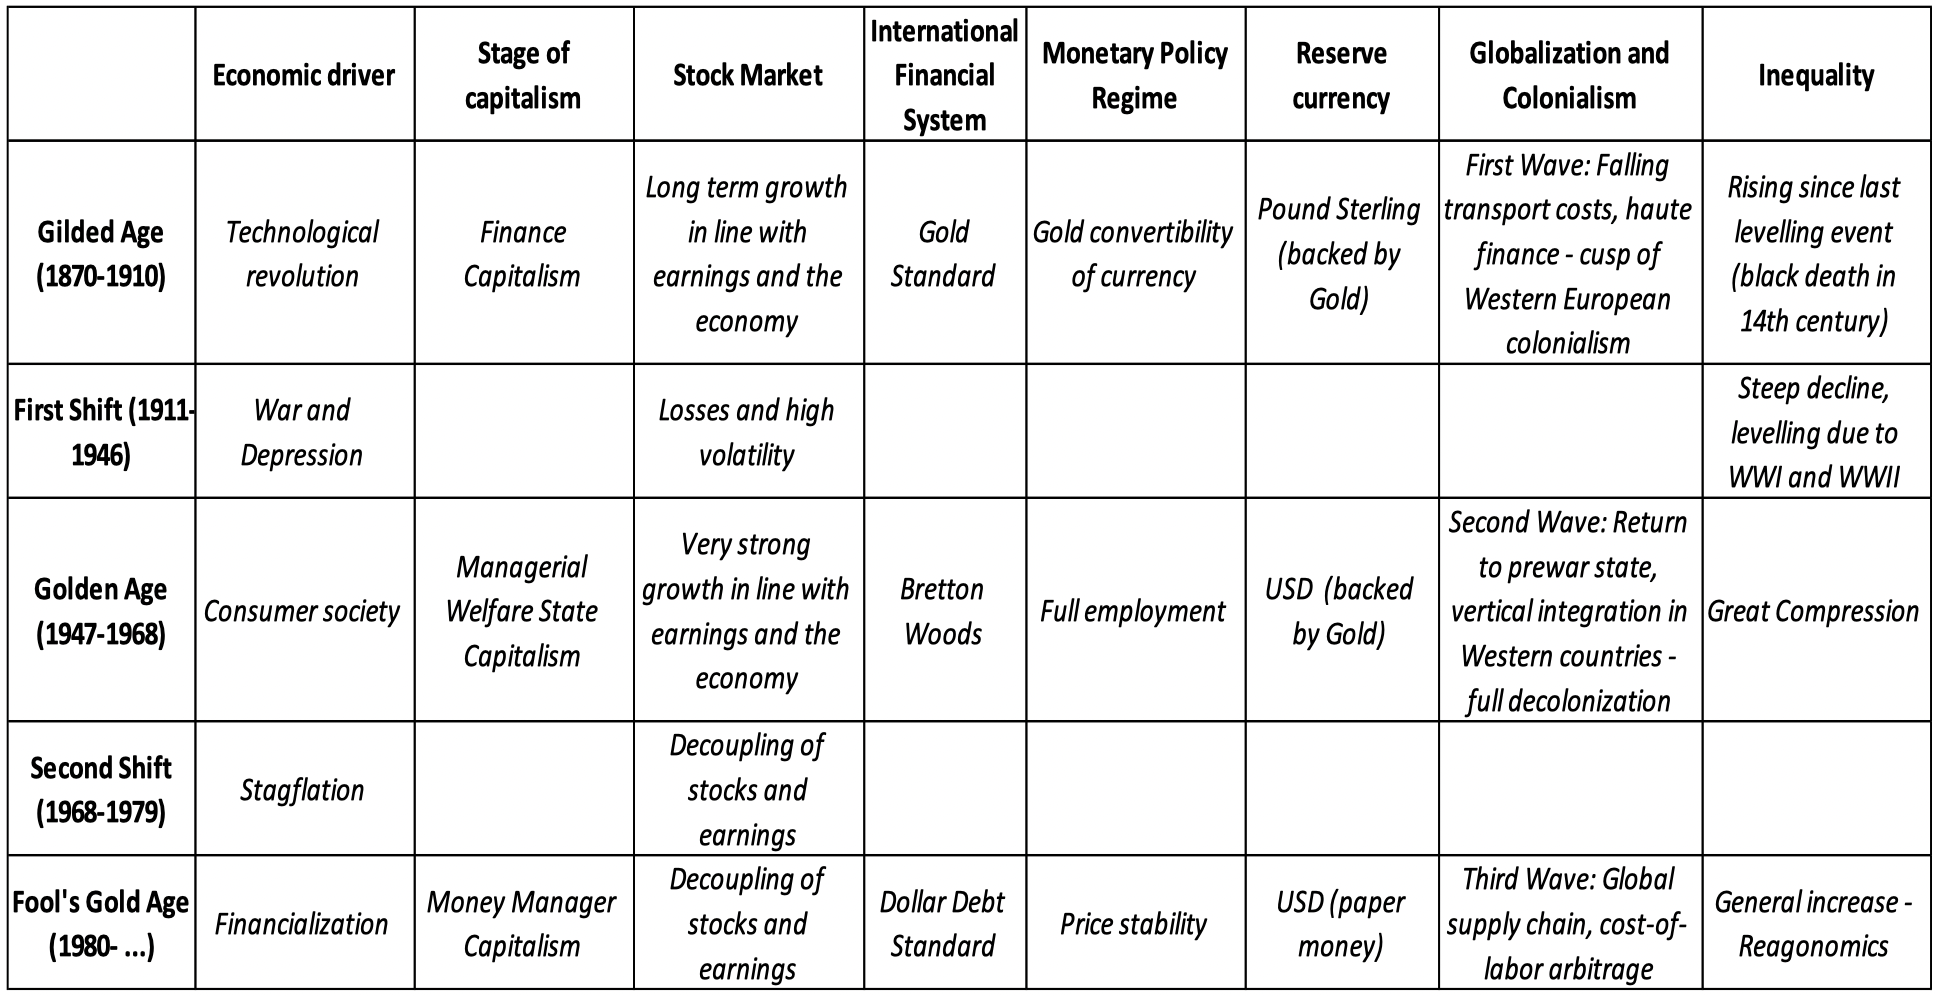
\includegraphics[width=15cm]{../images/EnpRisk_Fig10-1}
    \centering
\end{figure}

\section{History of Discovery, Invention and Innovation}

\subsection{Nature of Economic Growth}

The output of an economy, in a specific country, over a certain period, is measured in terms of the \textbf{Gross Domestic Product (GDP).} GPD gives the monetary value of final goods and services - that are those bought by the final user. The simplest measure of \textit{economic growth} is the annual increase of the GDP. But it's better to correct for changes in inflation and population and use the annual increase of real GDP per capita as a proxy for economic growth.

GDP is a very \textit{crude measure:} it only counts transactions that can be given a monetary value. Following some examples of what is excluded from the GDP:

\begin{itemize}
    \item Unpaid household or voluntary work
    \item So-called externalities like environmental destruction and pollution
    \item Free digital goods like online search engines and new digital commons like Wikipedia or social media
\end{itemize}

GDP is a \textit{short-term measure:} it only considers monetary transactions and flows and as such totally \textit{ignores capital assets of all kinds} such as the depletion of resources or loss of biodiversity, nor does it account for the improvement, decay, or even destruction of infrastructure or the value of human and social capital.

Using modern data analysis techniques, Lera and Sornette proved that economic growth is \textit{bimodal:}

\begin{itemize}
    \item With one regime of expansion with strong growth, and another regime of consolidation with low growth or decline
    \item The system naturally switches between these two regimes in one single dynamical process
    \item In this view, growth and consolidation are two sides of the same coin
\end{itemize}

\paragraph{Things versus ideas} This, such as objects and goods, are rival:

\begin{itemize}
    \item As more people drive on a highway or use water for irrigation, there are fewer of these goods to go around
    \item To increase productivity of each person in economic system using things (like a computer), you need to give each person such a thing. Economic output per capita, under such conditions, is proportional to the capital per person
    \item In a closed economy, capital is subject to diminishing returns
\end{itemize}

On the other hand, ideas are non-rival:

\begin{itemize}
    \item As more people use the Pythagorean theorem or the Java programming language, there is not less and less of the idea to go around
    \item Idea are not depleted by use, and it is technologically feasible for any number of people to use and idea simultaneously once it has been invented
    \item Taking logs and derivatives, in the simplest case, the economic growth is proportional to the growth rate of the total stock of ideas
\end{itemize}

\textbf{Solow Model:}

\begin{figure}[H]
    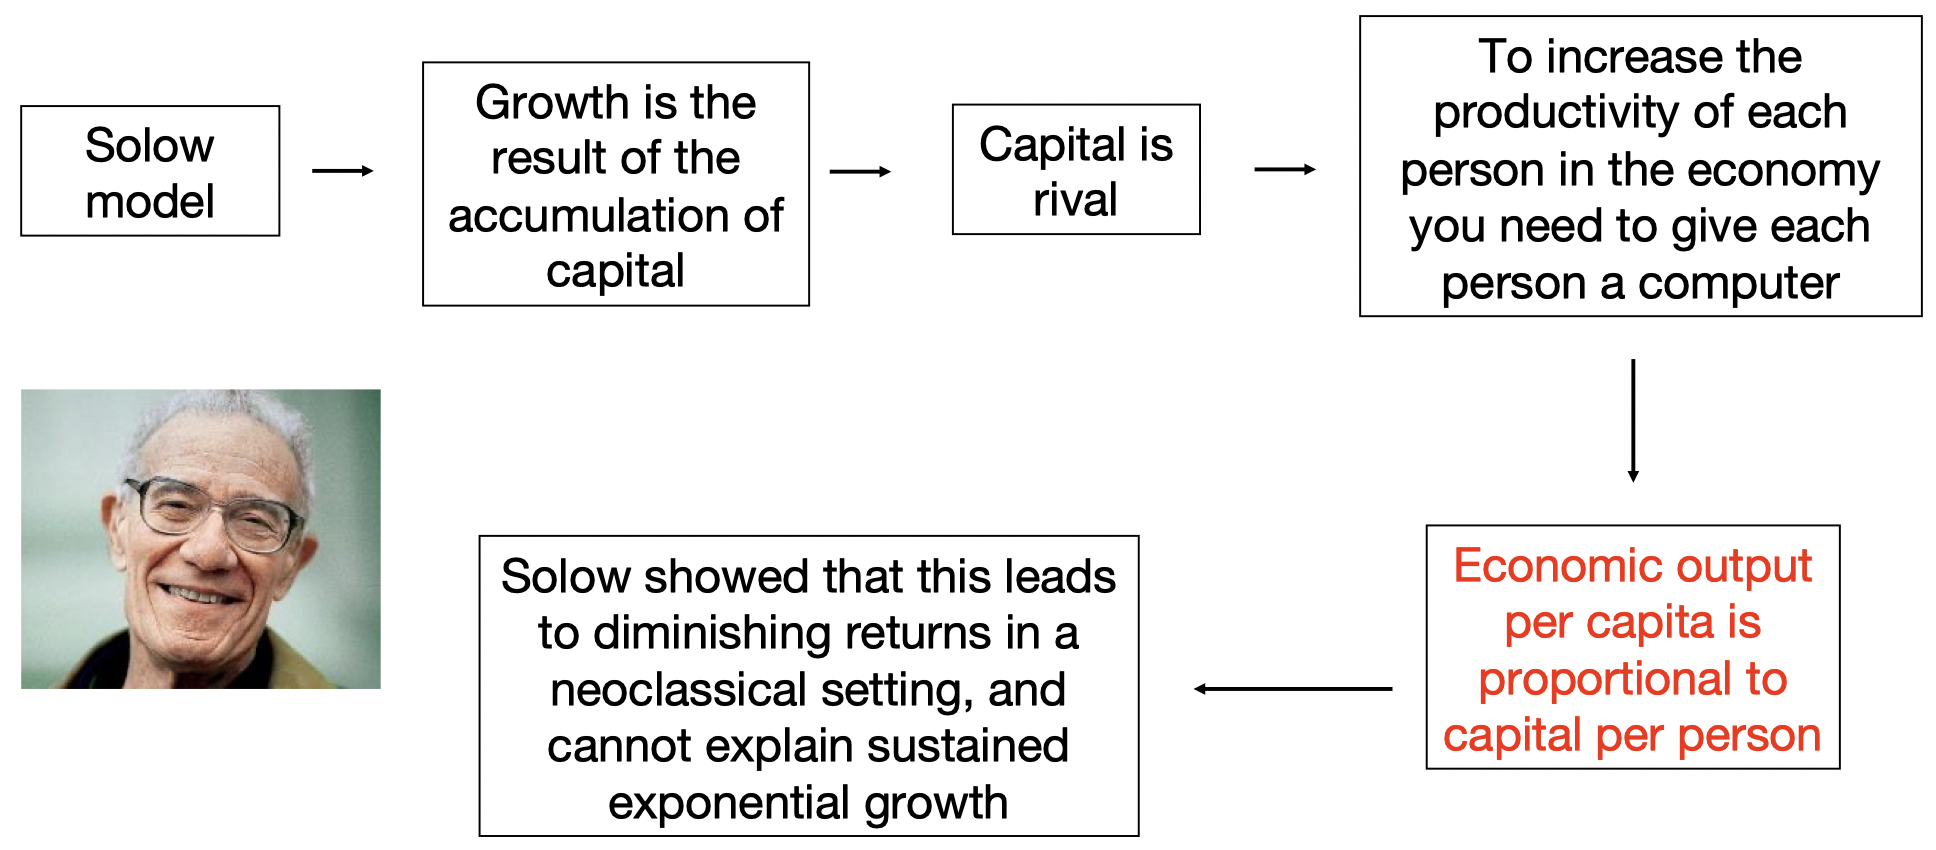
\includegraphics[width=15cm]{../images/EnpRisk_Fig10-2}
    \centering
\end{figure}

\textbf{Romer Model:}

\begin{figure}[H]
    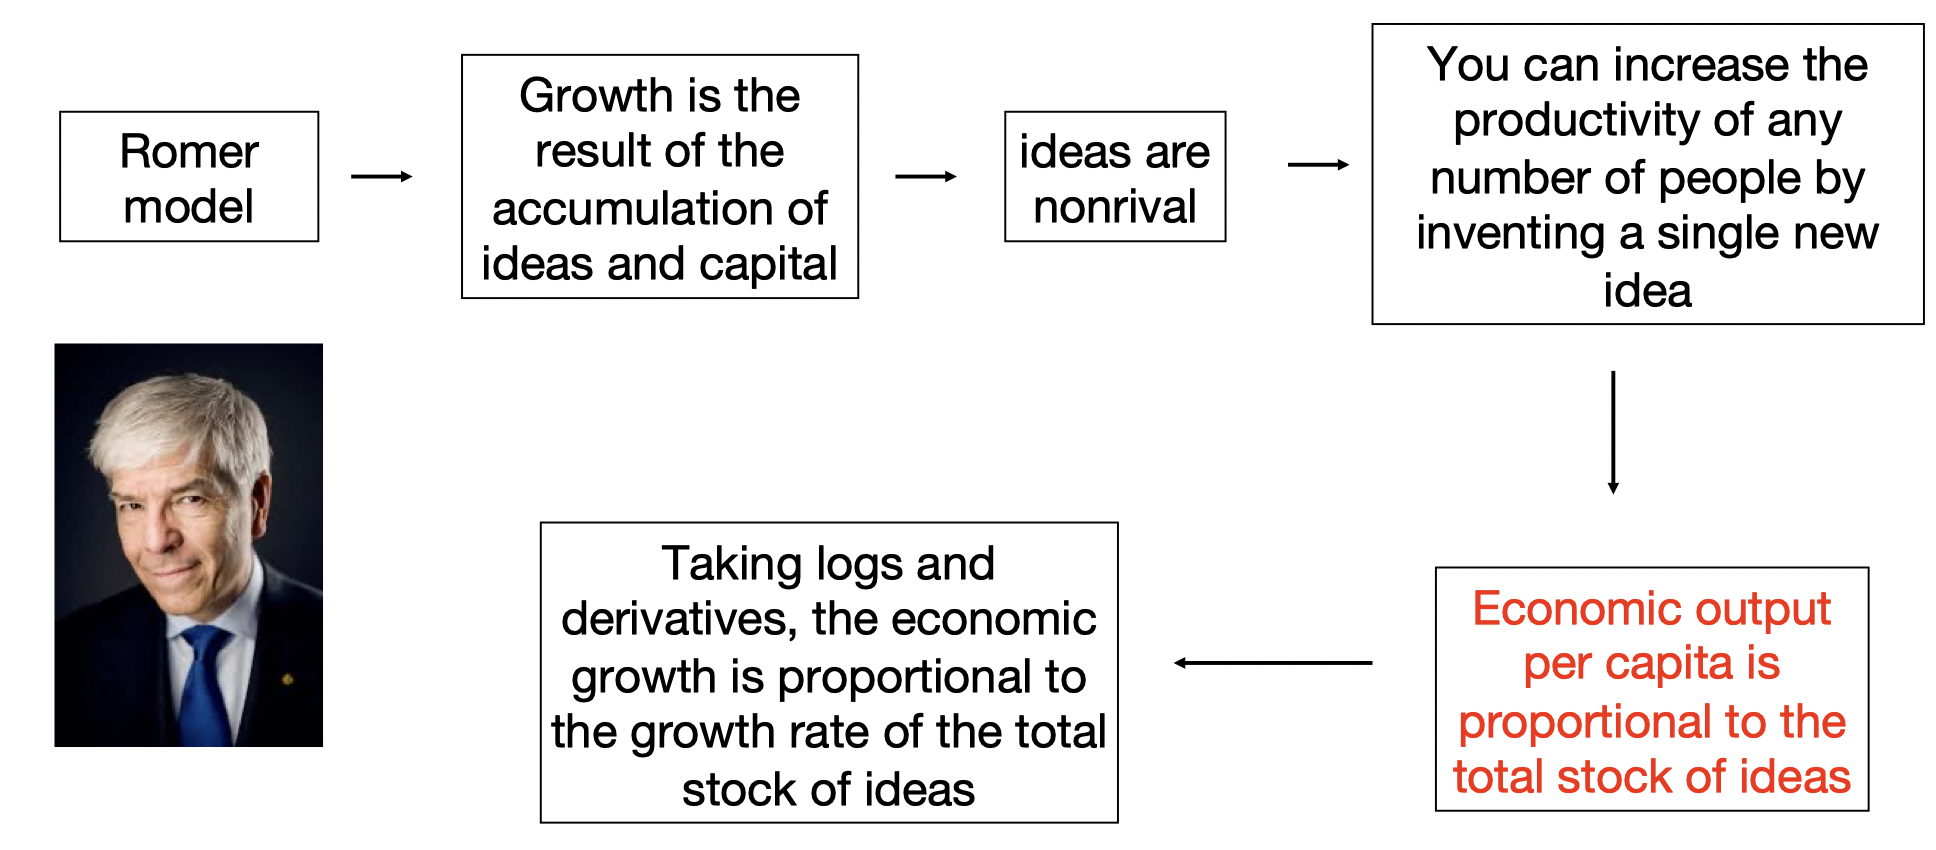
\includegraphics[width=15cm]{../images/EnpRisk_Fig10-3}
    \centering
\end{figure}

\end{document}